\documentclass{beamer}

\usefonttheme{professionalfonts} % using non standard fonts for beamer
\usefonttheme{serif} % default family is serif

\usepackage{hyperref}
%\usepackage{minted}
\usepackage{animate}
\usepackage{graphicx}
\def\Put(#1,#2)#3{\leavevmode\makebox(0,0){\put(#1,#2){#3}}}
\usepackage{colortbl}
\usepackage{tikz}
\usepackage{amssymb}
\usepackage{enumerate}
\usepackage{arydshln}
\usepackage{algorithm}
\usepackage{algpseudocode}

\colorlet{lightred}{red!25}
\colorlet{lightgreen}{green!25}


\newcommand\blfootnote[1]{%

  \begingroup

  \renewcommand\thefootnote{}\footnote{#1}%

  \addtocounter{footnote}{-1}%

  \endgroup

}

\makeatletter

%%%%%%%%%%%%%%%%%%%%%%%%%%%%%% Textclass specific LaTeX commands.

 % this default might be overridden by plain title style

 \newcommand\makebeamertitle{\frame{\maketitle}}%

 % (ERT) argument for the TOC

 \AtBeginDocument{%

   \let\origtableofcontents=\tableofcontents

   \def\tableofcontents{\@ifnextchar[{\origtableofcontents}{\gobbletableofcontents}}

   \def\gobbletableofcontents#1{\origtableofcontents}

 }

%%%%%%%%%%%%%%%%%%%%%%%%%%%%%% User specified LaTeX commands.

\usetheme{Malmoe}

% or ...

\useoutertheme{infolines}

\addtobeamertemplate{headline}{}{\vskip2pt}

\setbeamercovered{transparent}

% or whatever (possibly just delete it)

\makeatother

\begin{document}
\title[PFLOCK report]{PFLOCK Report}
\author[AC]{Andres Calderon}
\institute[Winter'20]{University of California, Riverside}
\makebeamertitle
\newif\iflattersubsect

\AtBeginSection[] {
    \begin{frame}<beamer>
    \frametitle{Outline} 
    \tableofcontents[currentsection]  
    \end{frame}
    \lattersubsectfalse
}

\AtBeginSubsection[] {
    \begin{frame}<beamer>
    \frametitle{Outline} 
    \tableofcontents[currentsubsection]  
    \end{frame}
}


\begin{frame}{Partition based join...}
    \begin{enumerate}
        \item Partition pointset A and B using the same set of grids (Quadtree grids).
        \item For pointset A, compute the position of each point according to a local grid with a predefined width.
        \item For pointset B, compute the position in the local grid AND manage replication.
        \item At each local grid, filter points which do not fulfill the distance condition.
        \item Merge back and remove possible duplicates.
    \end{enumerate}
\end{frame}

\begin{frame}{Partition based join...}{Global grids}
    \centering
    
\includegraphics[width=0.725\textwidth]{figures/GlobalGrids}
\end{frame}
\begin{frame}{Partition based join...}{Local grids}
    \centering
    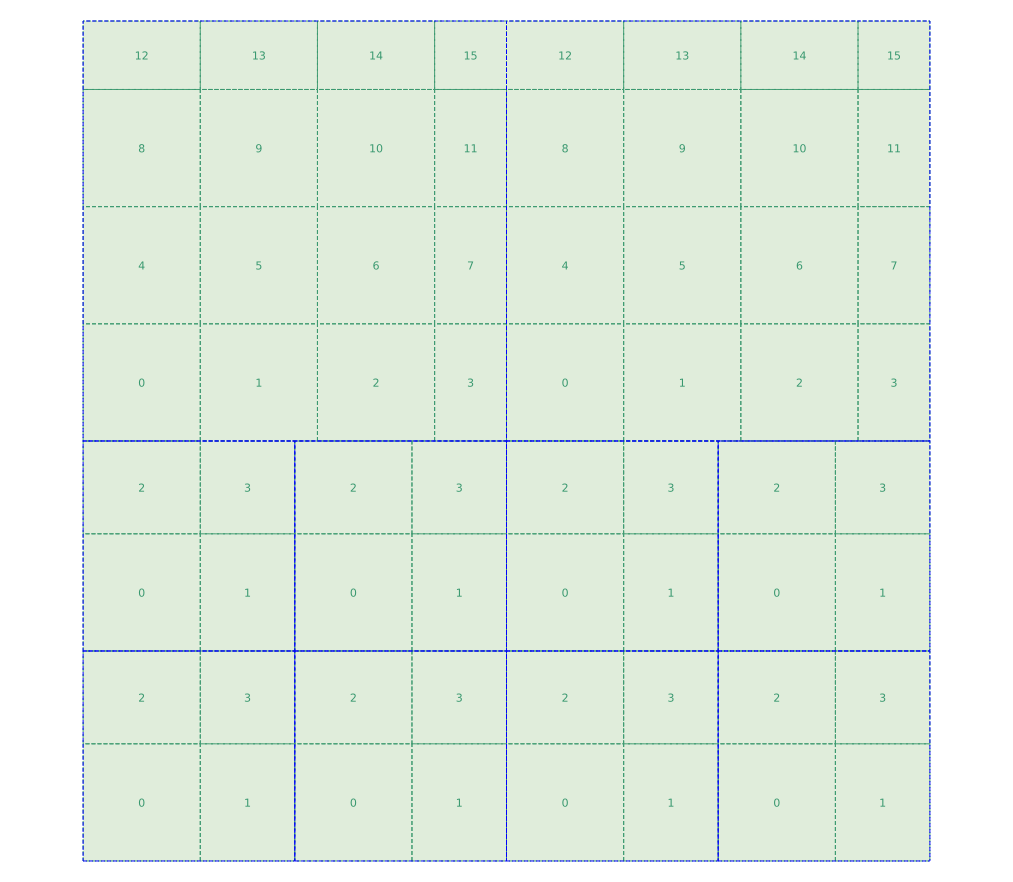
\includegraphics[width=0.725\textwidth]{figures/LocalGrids}
\end{frame}
\begin{frame}{Partition based join...}{Pointset A}
    \centering
    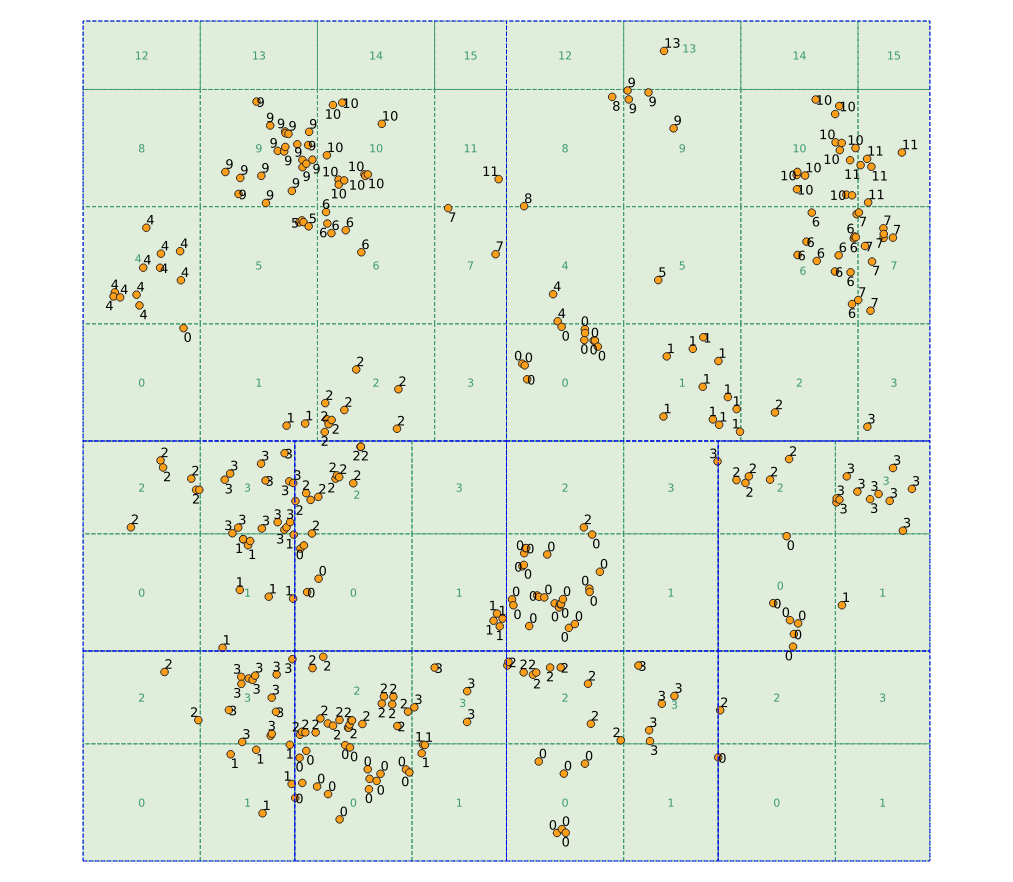
\includegraphics[width=0.725\textwidth]{figures/PointsetA}
\end{frame}
\begin{frame}{Partition based join...}{Pointset B (replication)}
    \centering
    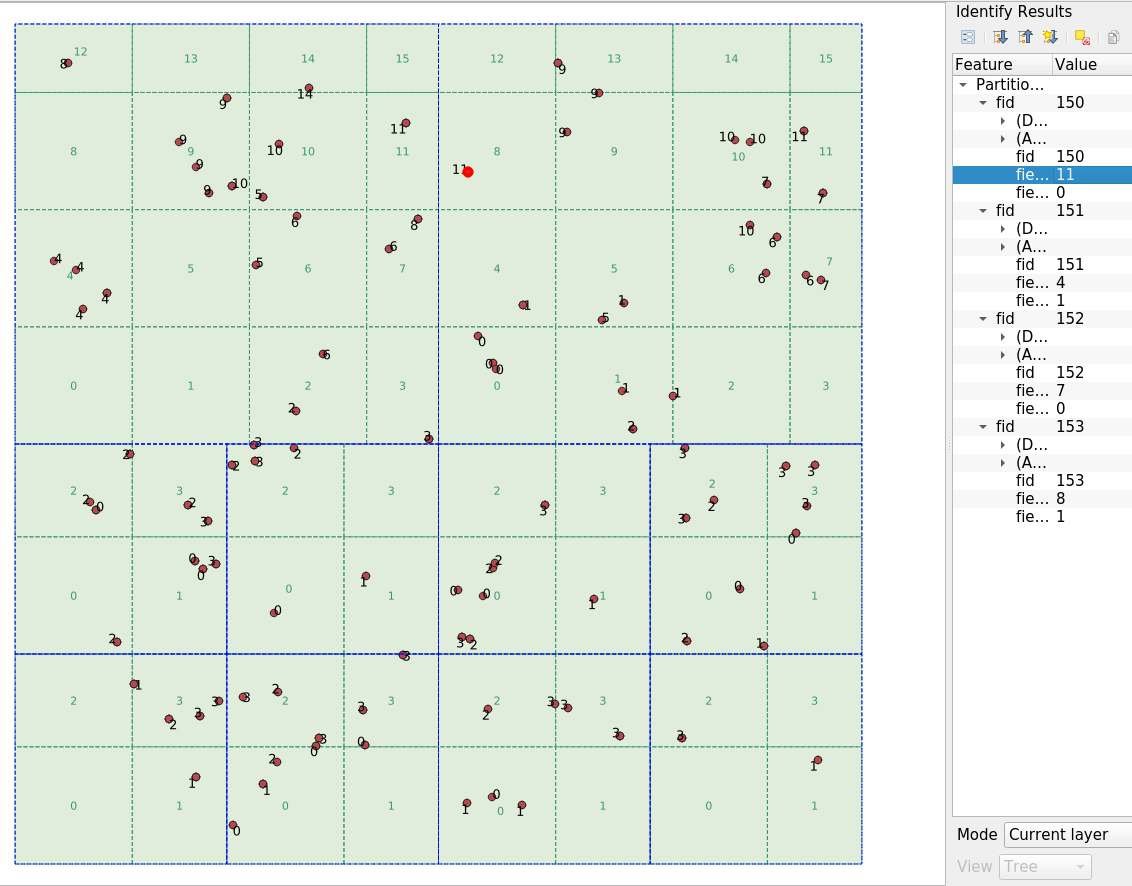
\includegraphics[trim={0 0 0 2mm},clip, width=0.8\textwidth]{figures/PointsetBa}
\end{frame}
\begin{frame}{Partition based join...}{Pointset B }
    \centering
    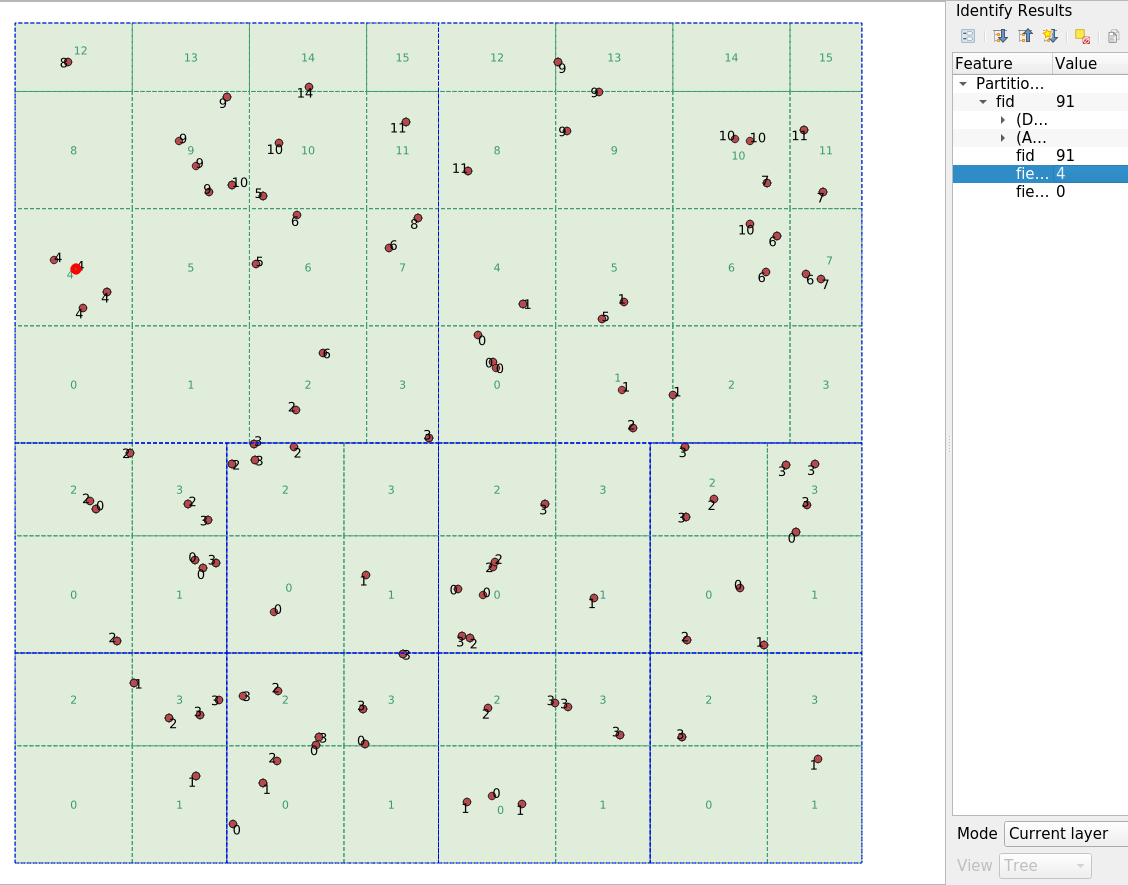
\includegraphics[trim={0 0 0 2mm},clip, width=0.8\textwidth]{figures/PointsetBb}
\end{frame}

\begin{frame}{What's next?}
    \begin{itemize}
        \item Currently working on the merge back and deduplication strategies...
        \item Perform more robust tests...
    \end{itemize}
\end{frame}

\end{document}
